\documentclass[12pt,journal,compsoc,onecolumn]{IEEEtran}
\usepackage{graphicx}
\usepackage{cite}
\usepackage{url}
\usepackage{caption}

\providecommand{\PSforPDF}[1]{#1}
\newcommand{\um} {$\mu$m}


\newcommand\MYhyperrefoptions{bookmarks=true,bookmarksnumbered=true,
pdfpagemode={UseOutlines},plainpages=false,pdfpagelabels=true,
colorlinks=true,linkcolor={black},citecolor={black},pagecolor={black},
urlcolor={black},
pdftitle={Third interim report},%<!CHANGE!
pdfsubject={Typesetting},%<!CHANGE!
pdfauthor={Carsten Bruns \& Jakob Toft},%<!CHANGE!
pdfkeywords={High-speed communication, Voltage-mode driver, Low-power 10GB/s}}%<^!CHANGE!

% correct bad hyphenation here
\hyphenation{op-tical net-works semi-conduc-tor}

\usepackage[]{units}
\usepackage{graphicx}
\usepackage{subfigure}

\usepackage{epstopdf}

\usepackage{pgfplots} 
\usepgfplotslibrary{external}
\tikzexternalize

\usepackage{float}

\begin{document}
%
% paper title
% can use linebreaks \\ within to get better formatting as desired
\title{Design, Analysis and Simulation of an I/O Link\\Second interim report}

\author{Carsten Bruns
        \& Jakob Toft% <-this % stops a space

%\IEEEcompsoctitleabstractindextext{%
%\begin{abstract}
%\boldmath
%The abstract goes here.
%\end{abstract}


% Note that keywords are not normally used for peerreview papers.
\begin{IEEEkeywords}
High-Speed Data Links, Low-Power 10Gb/s link.
\end{IEEEkeywords}}


% make the title area
\maketitle

\IEEEdisplaynotcompsoctitleabstractindextext
\IEEEpeerreviewmaketitle

dfk\cite{rajesh2011a} %TODO remove
%\section{Choice of the citcuit topology}

\IEEEPARstart{T}{odo} write sth here! \cite{cressler2007a}
\section{Transmitter schematics}

%TODO explain layering
%TODO explain sizing!! and give the values!

\begin{figure}[ht]
  \centering
  {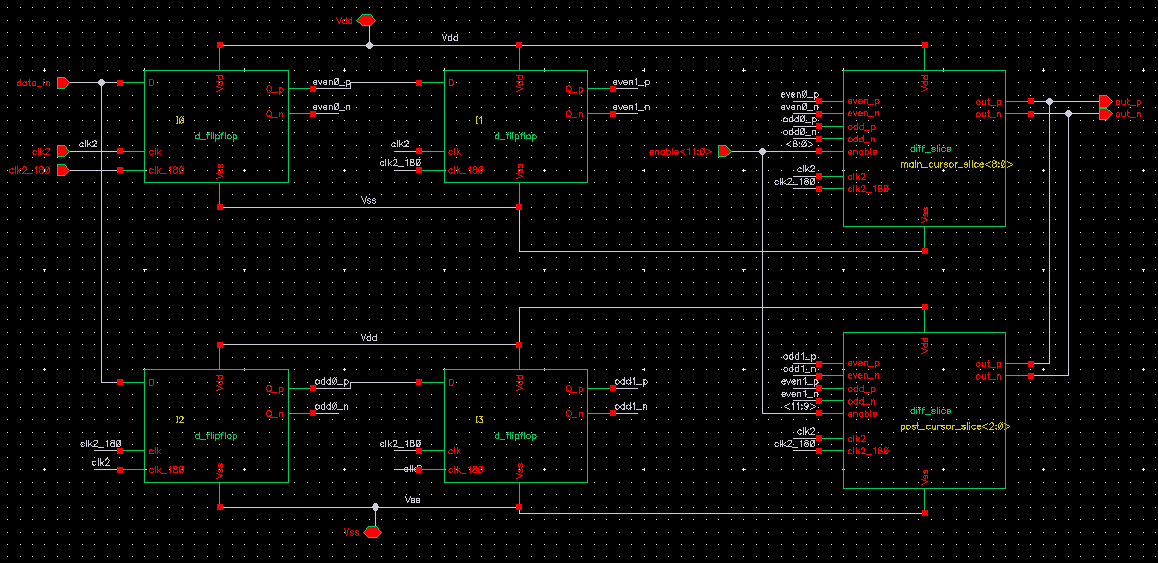
\includegraphics[scale=0.55]{img/transmitter.png}}
  \caption{Transmitter top level circuit}
  \label{fig:top_level}
\end{figure}

\begin{figure}[ht]
  \centering
  \subfigure[Differential slice]
  {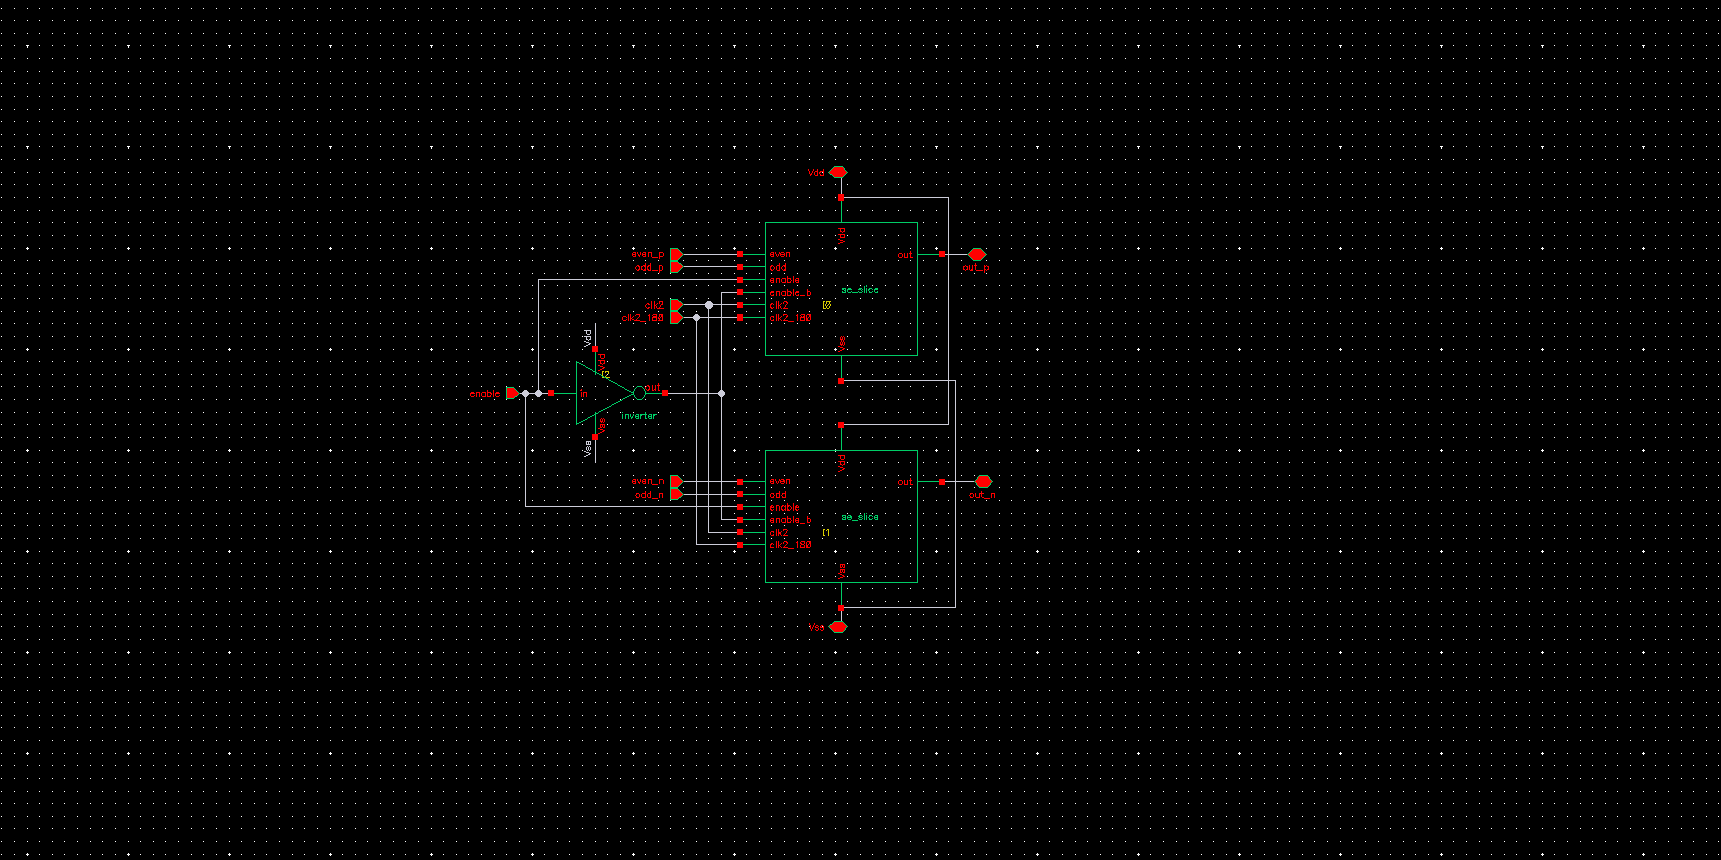
\includegraphics[scale=0.6]{img/diff_slice.png}}
  \subfigure[Single-ended slice]
  {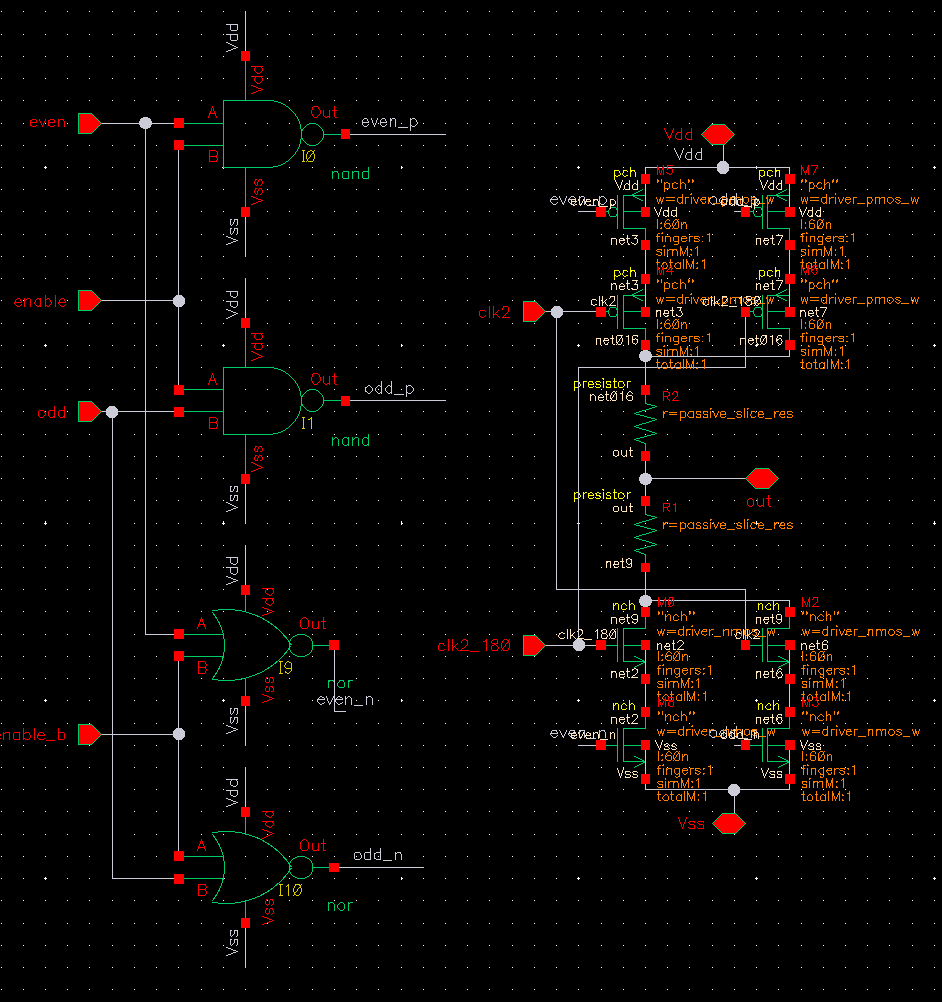
\includegraphics[scale=0.5]{img/se_slice.png}}
  \caption{Slice circuits}
  \label{fig:slices}
\end{figure}

\begin{figure}[ht]
  \centering
  {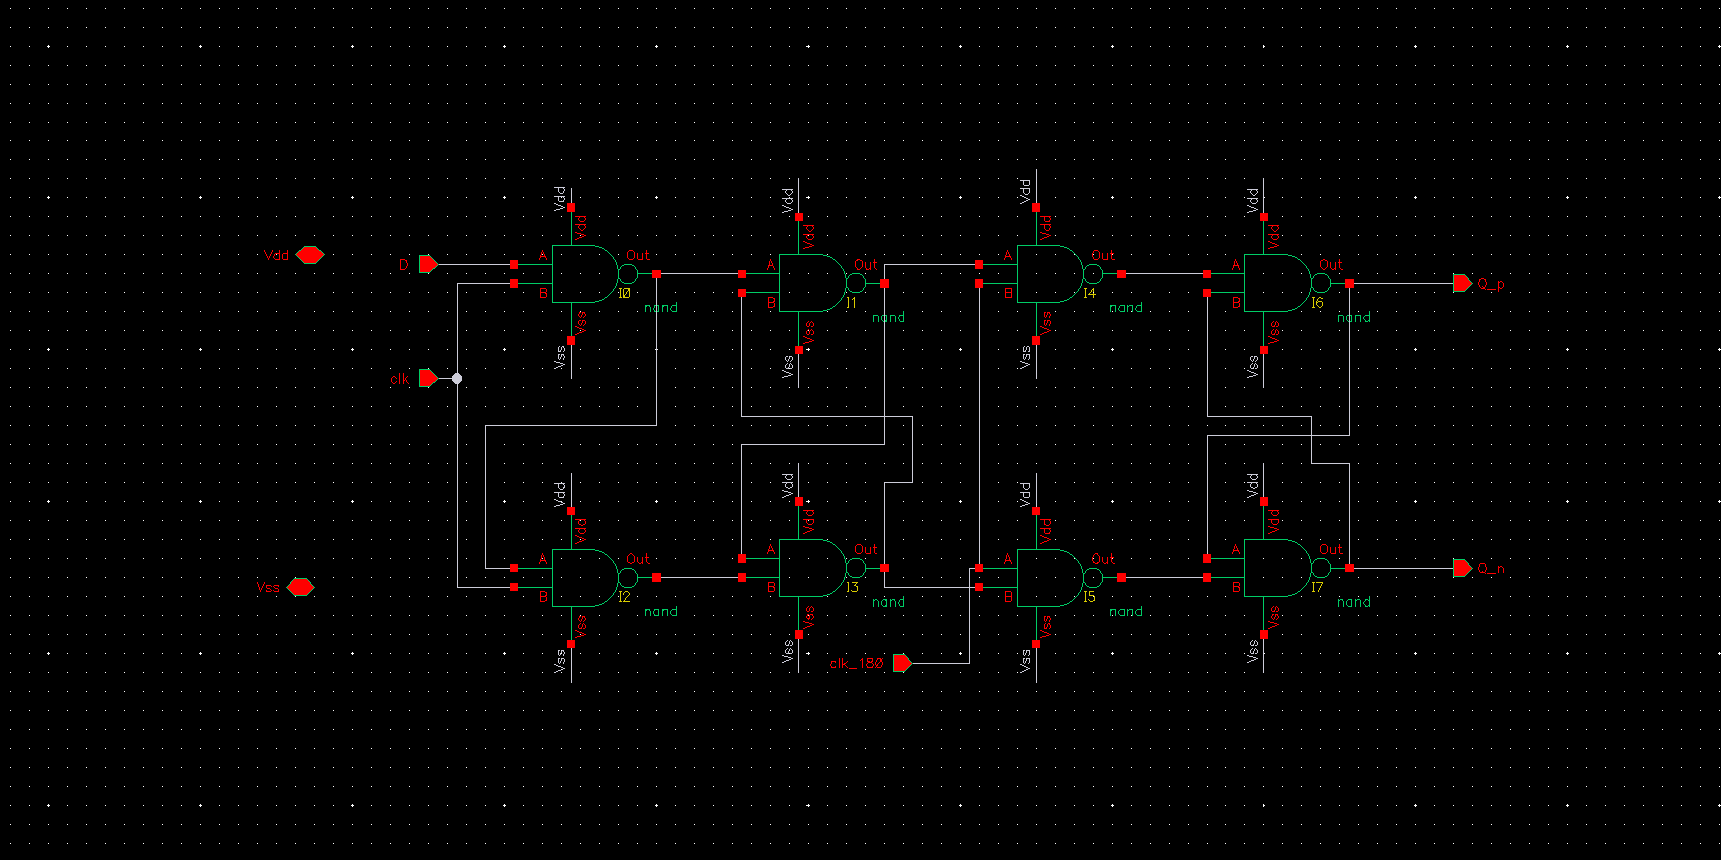
\includegraphics[scale=0.47]{img/flipflop.png}}
  \caption{D-Flipflop}
  \label{fig:flipflop}
\end{figure}

\begin{figure}[ht]
  \centering
  \subfigure[Inverter]
  {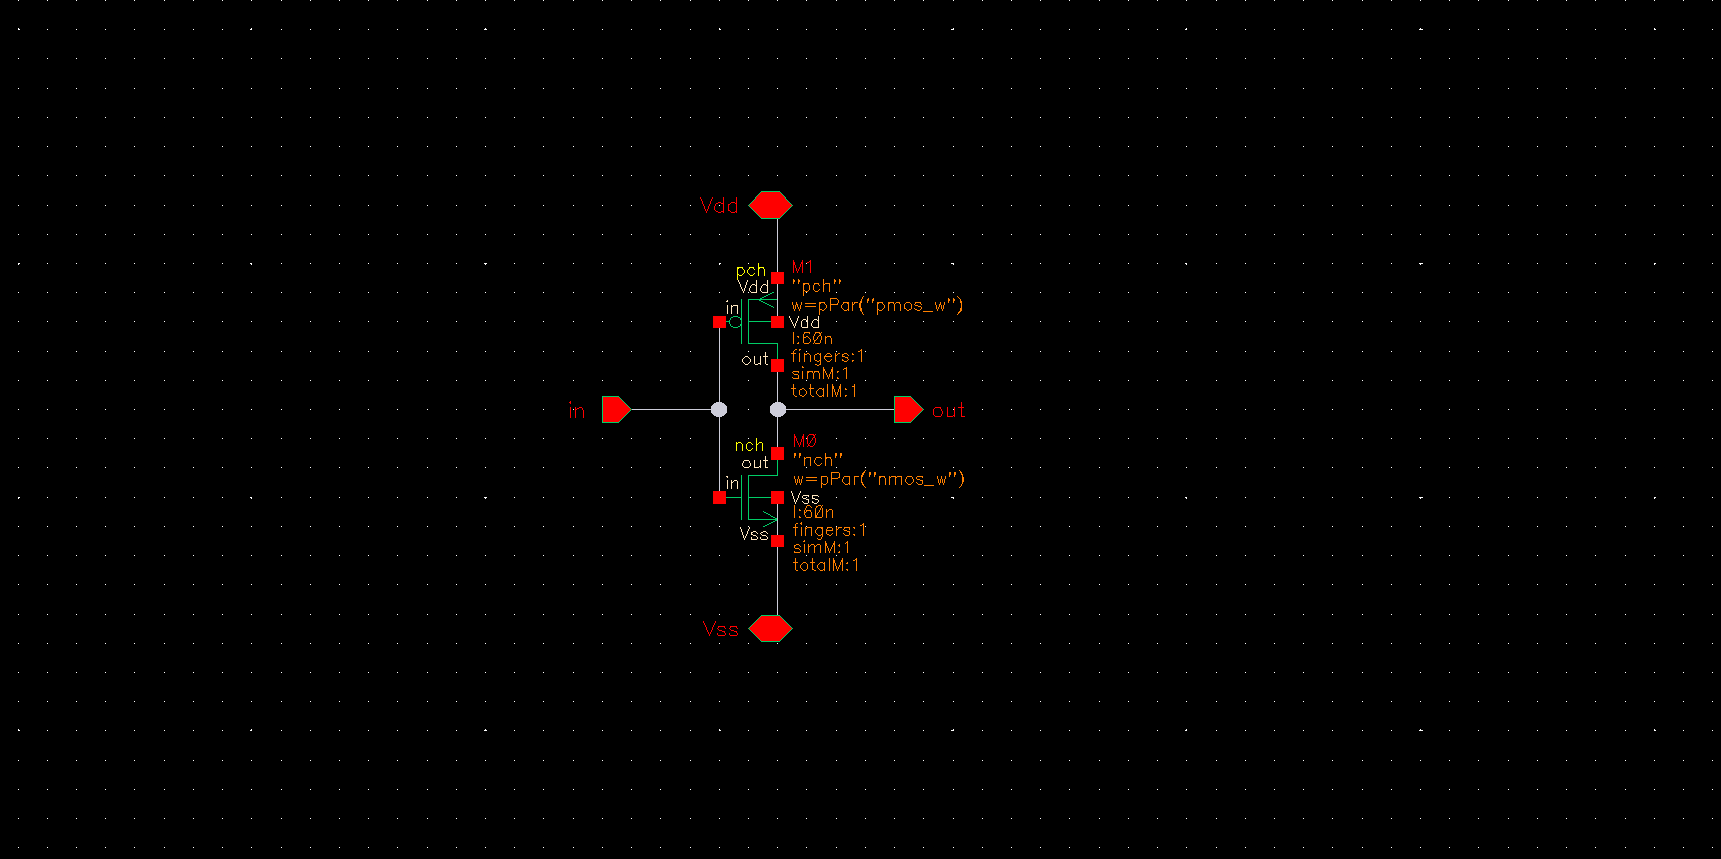
\includegraphics[scale=0.5]{img/inverter.png}}
  \subfigure[NAND gate]
  {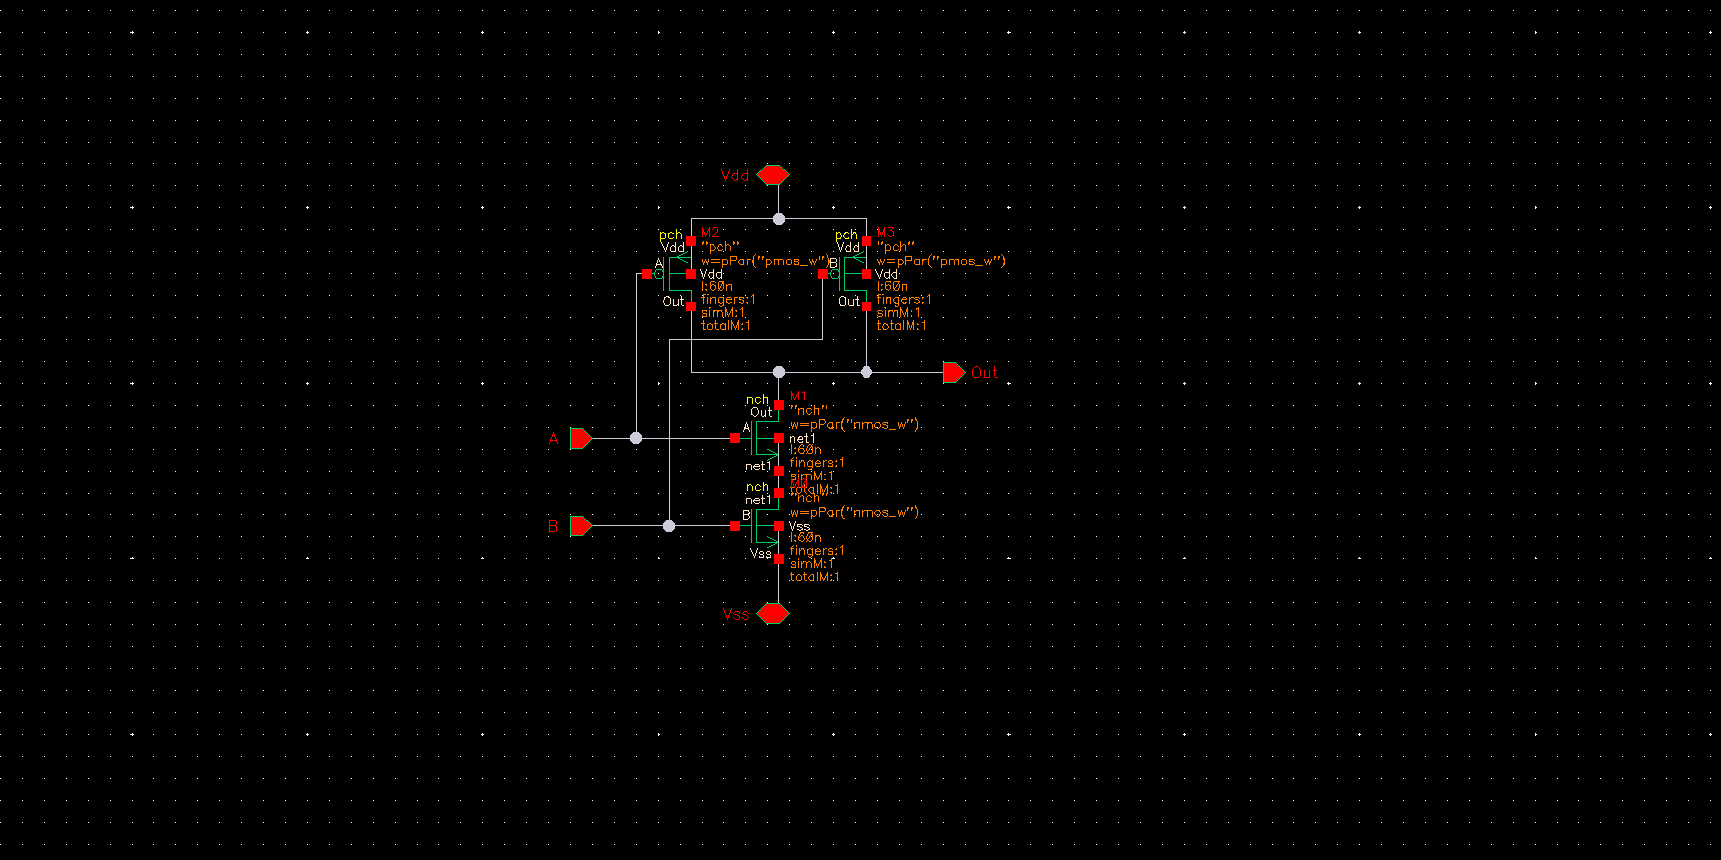
\includegraphics[scale=0.5]{img/nand.png}}
  \subfigure[NOR gate]
  {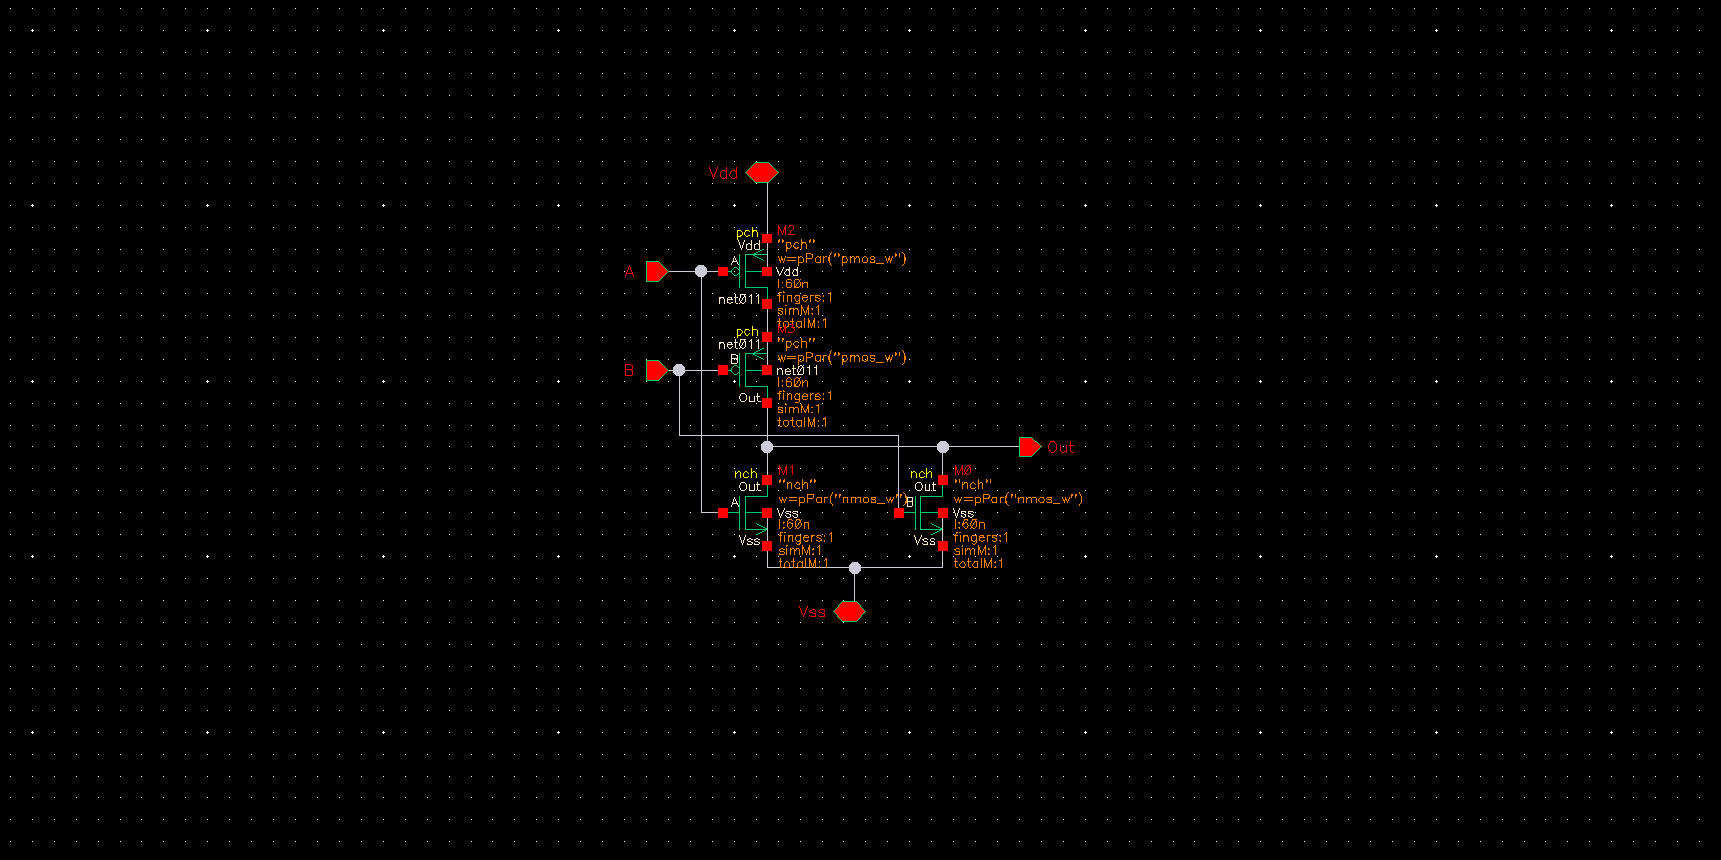
\includegraphics[scale=0.5]{img/nor.png}}
  \caption{Simple gate circuits}
  \label{fig:gates}
\end{figure}
\section{Impedance tuning}

\IEEEPARstart{T}{odo} write sth here!

%TODO tuning range graph
%\section{Performance results}

\IEEEPARstart{T}{odo} write sth here!

%TODO table with performance/specs



% Can use something like this to put references on a page
% by themselves when using endfloat and the captionsoff option.
\ifCLASSOPTIONcaptionsoff
  \newpage
\fi

\newpage
\section{Bibliography}
\bibliography{biblio}{}
\bibliographystyle{plain}


\end{document}


